\documentclass[border=0.2cm]{standalone}
\usepackage{tikz}
\usepackage{graphicx}
\usetikzlibrary{shapes.geometric} % for the hexagon
\usetikzlibrary{shapes} % for the hexagon
\usepackage{xcolor}

\definecolor{newgreen}{HTML}{0CFFBE}

\begin{document}
\begin{tikzpicture}[scale=2.5]
  % Create a clipping mask in the shape of a hexagon
  \begin{scope}

    \clip [scale=.99] ( {cos(60*1)} , {sin(60*1)} )
    -- ( {cos(60*2)} , {sin(60*2)} )
    -- ( {cos(60*3)} , {sin(60*3)} )
    -- ( {cos(60*4)} , {sin(60*4)} )
    -- ( {cos(60*5)} , {sin(60*5)} )
    -- ( {cos(60*6)} , {sin(60*6)} )
    -- cycle;

    % \node at (0,0) {\includegraphics[height=4.5cm]{wheatfield.jpg}};
    \node at (0,0) {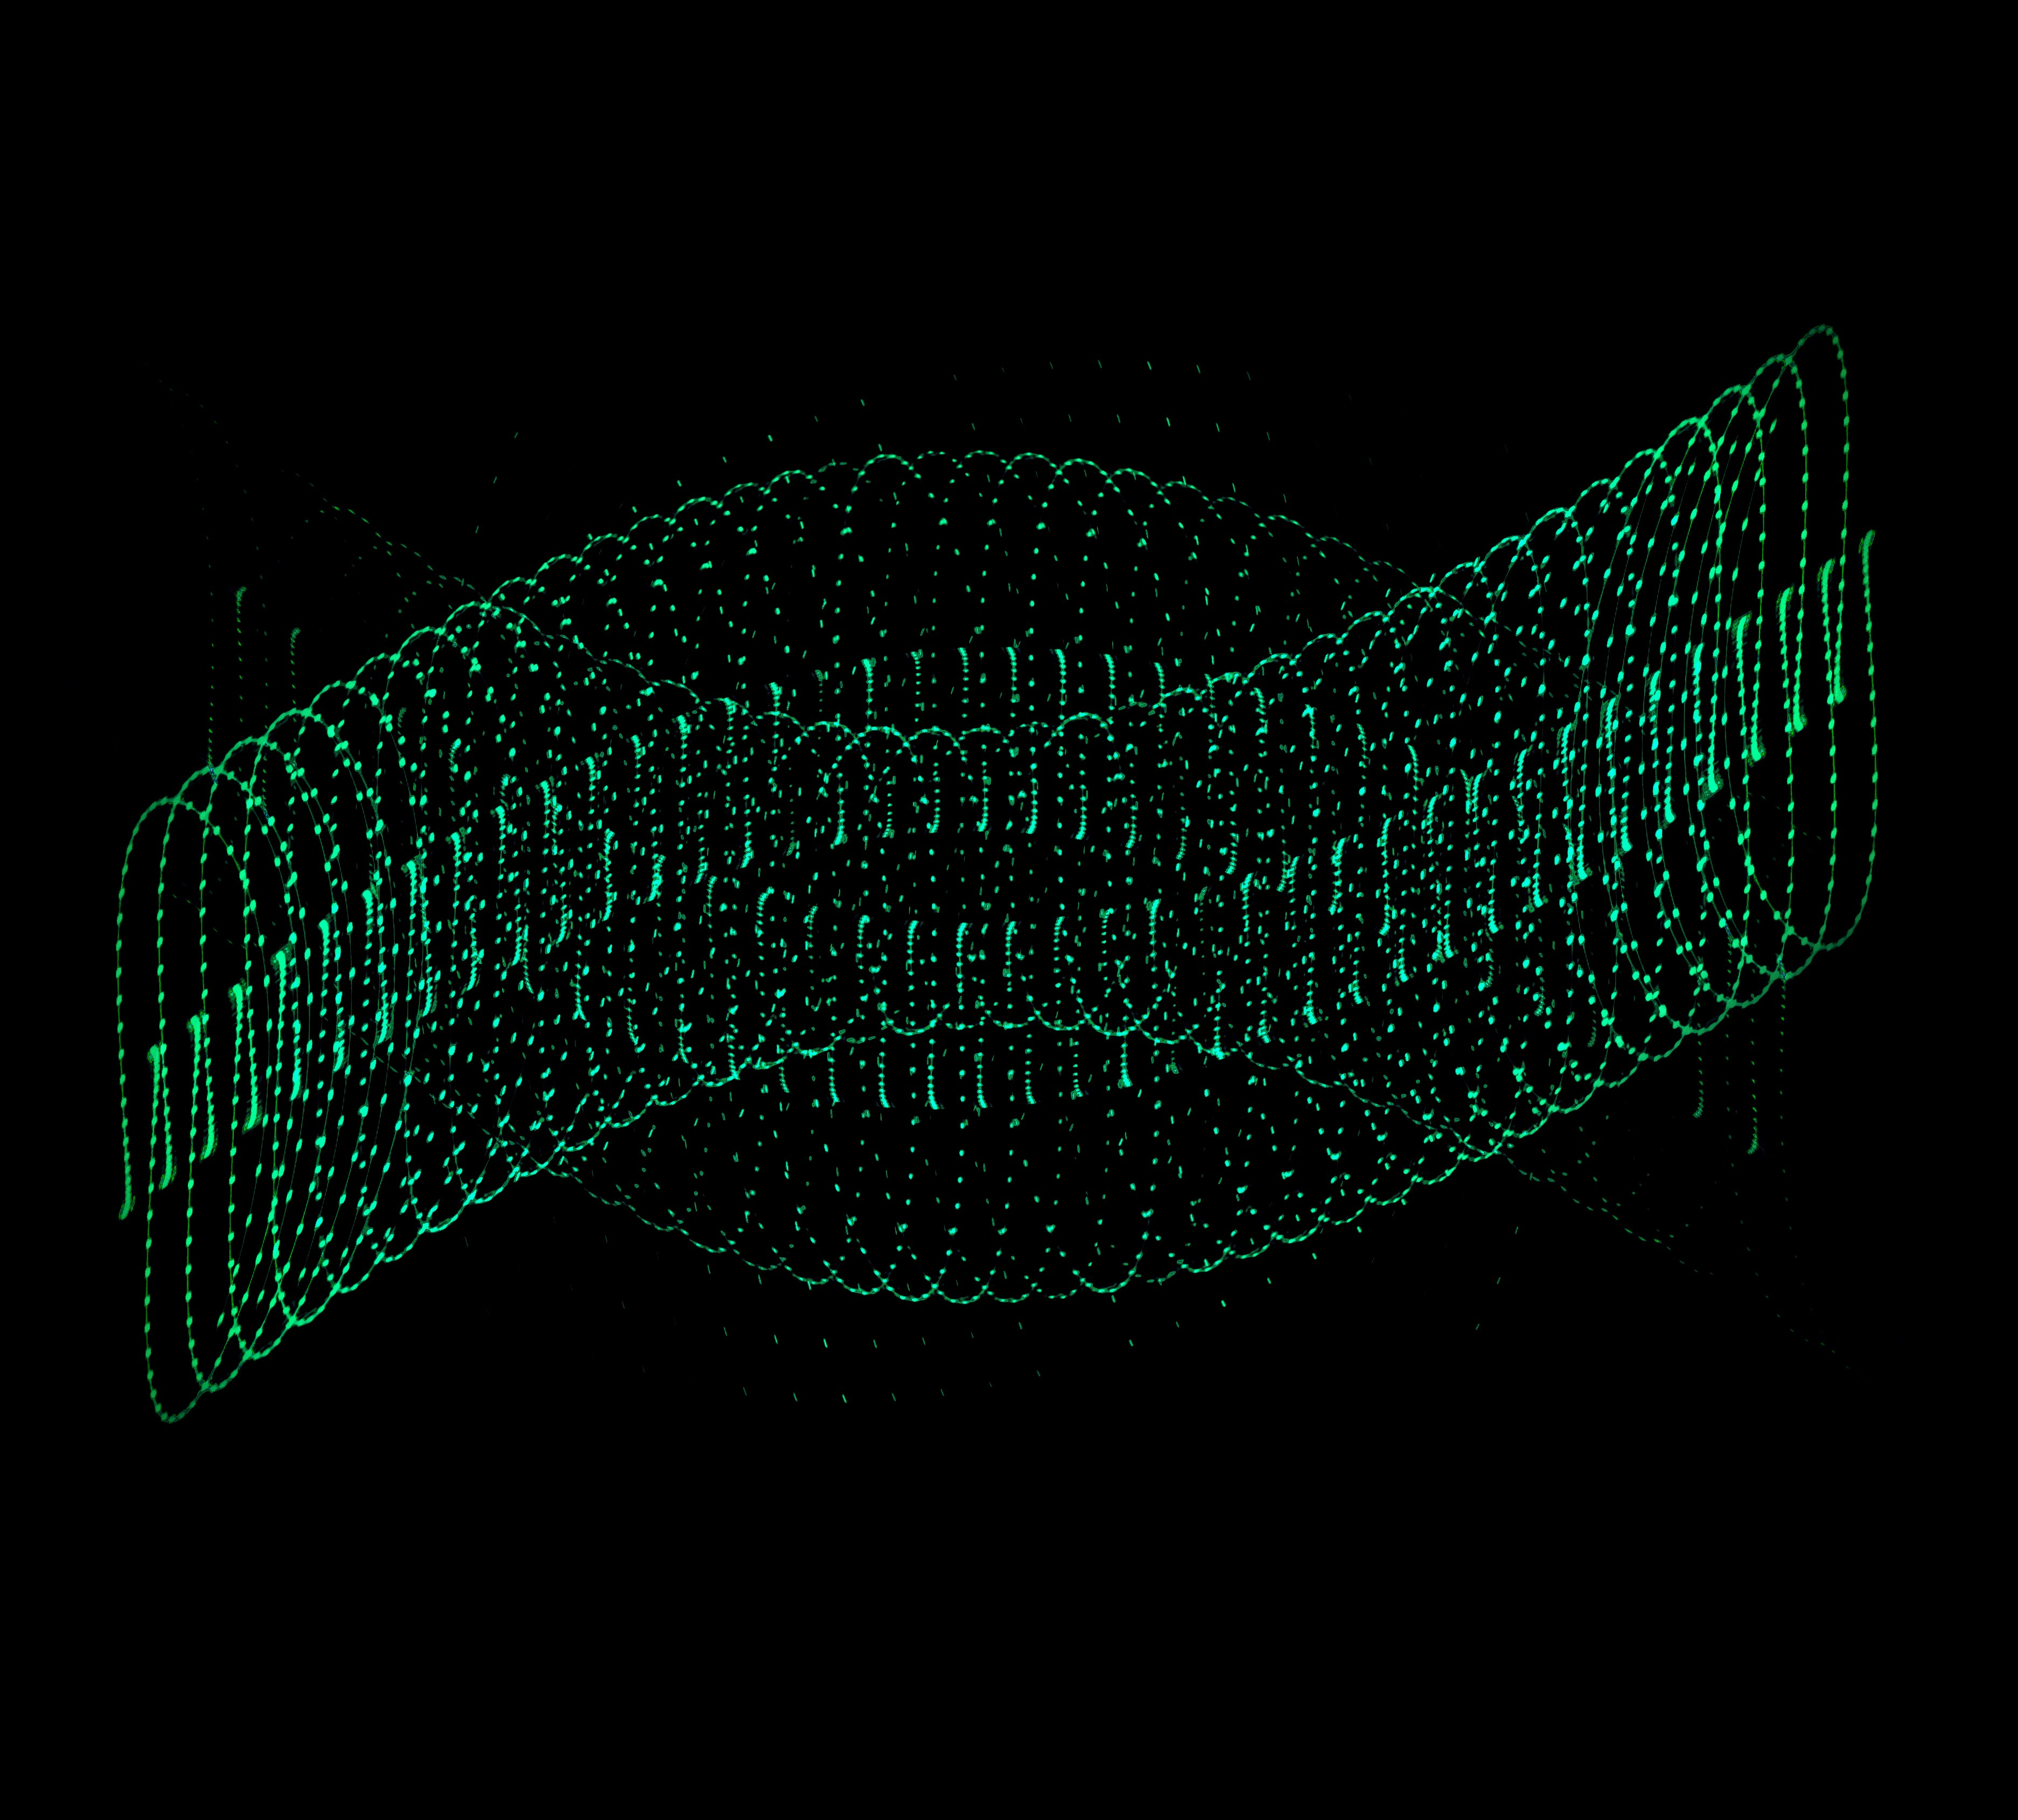
\includegraphics[width=5cm]{mariola-grobelska.jpg}};
    
  \end{scope}
  
  % Optionally, draw the hexagon outline to emphasize the mask
  \draw[black, thick] (0,0) node[regular polygon, regular polygon sides=6, inner sep = 1.5cm] {};
  \node[ultra thick, regular polygon, draw, regular polygon sides = 6, inner sep=1.55cm] (p) at (0, 0) {};
  \node[ultra thick, regular polygon, draw, regular polygon sides = 6, color = newgreen!40!black, inner sep=1.52cm] (p) at (0, 0) {};
  
  % Add text at the bottom of the figure
  % \node [scale=1.05, rotate = 0] at (0,-.76) {\textbf{\texttt{\{Simulacron3\}}}};
  \node [scale=1.05, rotate = 0, color=newgreen] at (0,-.65) {\textbf{\texttt{\{Simulacron3\}}}};
\end{tikzpicture}
\end{document}

